\documentclass[10pt]{beamer}
\usepackage[T1,T2A]{fontenc}
\usepackage[utf8]{inputenc}
\usepackage{hyperref}
\hypersetup{unicode=true}
\usepackage{fontawesome}
\usepackage{graphicx}
\usepackage[english,russian]{babel}

\usepackage[T1]{fontenc}
\usepackage{fontawesome}
\usepackage{PTSans} 
\mode<presentation>
{
  \usetheme[progressbar=foot,numbering=fraction,background=light]{metropolis} 
  \usecolortheme{default}
  \usefonttheme{default}
  \setbeamertemplate{navigation symbols}{}
  \setbeamertemplate{caption}[numbered]
} 

\let\textttorig\texttt
\renewcommand<>{\texttt}[1]{%
  \only#2{\textttorig{#1}}%
}

\usepackage{minted}

\usepackage{xcolor}
\definecolor{codecolor}{HTML}{FFC300}

\usepackage{tcolorbox}
\tcbuselibrary{most,listingsutf8,minted}

\tcbset{tcbox width=auto,left=1mm,top=1mm,bottom=1mm,
right=1mm,boxsep=1mm,middle=1pt}

\newtcblisting{myr}[1]{colback=codecolor!5,colframe=codecolor!80!black,listing only, 
minted options={numbers=left, style=tcblatex,fontsize=\tiny,breaklines,autogobble,linenos,numbersep=3mm},
left=5mm,enhanced,
title=#1, fonttitle=\bfseries,
listing engine=minted,minted language=r}

\definecolor{mygreen}{HTML}{37980D}
\definecolor{myblue}{HTML}{0D089F}
\definecolor{myred}{HTML}{98290D}

\usepackage{listings}

\lstdefinelanguage{XML}
{
  morestring=[b]",
  morecomment=[s]{<!--}{-->},
  morestring=[s]{>}{<},
  morekeywords={ref,xmlns,version,type,canonicalRef,metr,real,target}
}

\lstdefinestyle{myxml}{
language=XML,
showspaces=false,
showtabs=false,
basicstyle=\ttfamily,
columns=fullflexible,
breaklines=true,
showstringspaces=false,
breakatwhitespace=true,
escapeinside={(*@}{@*)},
basicstyle=\color{mygreen}\ttfamily,
stringstyle=\color{myred},
commentstyle=\color{myblue}\upshape,
keywordstyle=\color{myblue}\bfseries,
}


% ------------------------------------------------------------------------------
% The Document
% ------------------------------------------------------------------------------
\title{Разработка приложения <<Игра 2048>>}
\subtitle{Отчет о проектной работе по курсу <<Основы информатики и программирования>>}
\author{Дмитрий Сергеевич Мельников}
\date{11 июня 2021}

\begin{document}

\maketitle
\begin{frame}
  % Заголовок слайда
  \frametitle{Цель и задачи}
  \begin{block}{Цель работы}
    Разработа компьютерную программу, реализующую игру «2048» на языке С++ и qml
  \end{block}
  \begin{block}{Задачи}
  \begin{itemize}
   \item Проанализировать правила игры «2048», её оригинальную разработку, существующие аналоги. На основе проведенного анализа разработать концепцию требований к разрабатываемой программе.
    \item Разработать алгоритмы, необходимые для реализации игры «2048». Разработать макет пользовательского интерфейса.
    \item Разработать интерфейс и логику работы программы. Провести тестирование и отладку разработанной программы.
  \end{itemize}
  \end{block}
\end{frame}
 
\begin{frame}
    \frametitle{Этапы разработки приложения}
    \begin{enumerate}
        \item Создание макета игры.
        \item Разработка алгоритма игры при нажатии клавишь.
        \item Реализация кнопки "Новая игра" и "Выход".
        \item Разработка итогового дизайна.
    \end{enumerate}            
\end{frame}
    \begin{frame}
    \frametitle{helper.cpp}
   \begin{itemize}
\item newGame (Генерация новой игры)
\item right (Cмещение всех элементов вправо и если есть возможность сложение этих элементов)
\item left (Cмещение всех элементов влево и если есть возможность сложение этих элементов)
\item up (Cмещение всех элементов вверх и если есть возможность сложение этих элементов)
\item down (Cмещение всех элементов вниз и если есть возможность сложение этих элементов)
\end{itemize}
\end{frame}

\begin{frame}
\frametitle{Основны модули qml}
\item main.qml-Главный модуль графического интерфейса.
\item Brick.qml-Значение каждого из 16 квадратов.
\item Gameplay.qml-Графический интерфейс игрового поля.
\item Toolbar.qml-Графический интерфейс панели инструментов.
\end{frame}

\begin{frame}
\frametitle{Реализация}
\begin{column}{0.45\textwidth}
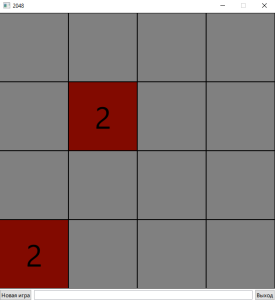
\includegraphics[width=\textwidth]{game2048.png}
\end{column}
\end{frame}
\begin{frame}
\frametitle{Заключение}
В результате проекта было разработана игра 2048.
\\

Получен опыт работы с библиотеками языка <<С++>>, а также опыт работы с <<Qt Quick>>.
\end{frame}

\begin{frame}
  \frametitle{}
  
{\Large\mbox{}\hfil Спасибо за внимание!}
  
\end{frame}
\end{document}
